\documentclass[12pt, titlepage]{article}

\usepackage{booktabs}
\usepackage{tabularx}
\usepackage{hyperref}
\hypersetup{
    colorlinks,
    citecolor=black,
    filecolor=black,
    linkcolor=red,
    urlcolor=blue
}
\usepackage[round]{natbib}
\usepackage{enumitem}
\usepackage{graphicx}
\usepackage[section]{placeins}
\usepackage{xltabular}
\usepackage{array, ltablex, caption, multirow, makecell}
\newcommand\nl{\newline}
\usepackage{array}
\usepackage{float}
\newcolumntype{P}[1]{>{\raggedright\arraybackslash}p{#1}}
\makeatletter
\def\itemlabel#1#2{\def\@currentlabel{#2}\phantomsection\label{#1}}
\title{SE 3XA3: Software Requirements Specification\\The Resume Shotgun}

\author{Team 5, Proper Mars Tribe
		\\ Gavin Jameson, jamesong
		\\ Jeremy Langner, langnerj
		\\ Sam Gorman, gormans
}

\date{\today}

%\input{../Comments}

\begin{document}

\maketitle

\pagenumbering{roman}
\tableofcontents
\listoftables
\listoffigures

\newpage

\pagenumbering{arabic}

This document describes the requirements for The Resume Shotgun. The template for the Software Requirements Specification (SRS) is a subset of the Volere template~\citep{RobertsonAndRobertson2012}. % If you make further modifications to the template, you should explicity state what modifications were made.

\section{Project Drivers}
% supersection

\subsection{The Purpose of the Project}
The modern job application process typically follows the same steps; applicants find potential employer's postings on a job board, determine if they think it's a good job, decide if they are a qualified candidate, and finally apply. This process is extremely tedious and mundane for most since it requires a substantial amount of reading through similar postings and similar processes for each.
The purpose of this project is to create a functioning application that allows the user to efficiently apply for multiple jobs on a variety of job board websites. The application utilizes user input from a resume to effectively match the user's experience/characteristics with potential job application descriptions. Once potential posting(s) are found, the user may confirm to submit an application for such position(s). The application will also allow for the user to upload auxiliary documents, such as cover letters and resumes. Multiple versions will be able to be uploaded in an attempt to tailor submissions for each job based on extracted key phrases. 

\subsection{The Stakeholders}
% supersection

\subsubsection{The Client}

The clients for this project, Dr Bokhari and the TA's for 3XA3, will be actively monitoring the project during its development and assuring that it follows their specifications. 

\subsubsection{The Customers}

The customers for this project consist of people searching for a job, specifically students looking to enter the workforce. The product suits the needs of these customers by casting a wide net and applying to all relevant positions. For the target customer base, the main issue with job searching is getting an interview for any relevant job, rather than the quality of the jobs applied for.  This is the issue that the Resume Shotgun aims to solve. 

\subsubsection{Other Stakeholders}

Using a template to apply to a job will inevitably make it less personal and less polished than it could be if one was to take the time to apply to jobs individually. Therefore, companies offering positions hold stakes in this project as the quality of the applications may go down due to using a more generalized template.

\subsection{Mandated Constraints}

\begin{itemize}
    \item Description: The product will run on modern machines with operating systems capable of executing Python code and installing required libraries.
	{\newline \emph{Rationale}: Python is a popular language with lots of documentation and support for any installing or execution issues the user may encounter.
	\newline \textbf{Fit Criterion}: Python supports all current and planned features, ensuring the product will be functional to the user.}
	
	\item Description: The product will run on any of the commonly used browsers (Chrome, Firefox, Safari).
	{\newline \emph{Rationale}: There are many widely used browsers with their own benefits/consequences. Allowing support for a variety of browsers lets the user choose their desired browser based on their own preferences and needs.
	\newline \textbf{Fit Criterion}: The product should require desired browser to be declared by the user to ensure proper functionality.}
\end{itemize}

\subsection{Naming Conventions and Terminology}

Some relevant naming conventions that will be used in this SRS and overall project are as follows:

\begin{itemize}
  \item OS: An operating system which is the integral software that binds the hardware to user capabilities.
  \item Windows: The operating system Microsoft Windows.
  \item GUI: Graphical User Interface, which is what the user will be using to interact with the program.
  \item PDF: Portable Document Format, a versatile format for text documents. Most basic text documents can be converted to this form.
  \item Python: The programming language that the program will be built in.
  \item Unittest: A module used to test python projects.
  \item Browser: The internet browser which the tool will use to access job boards. Common examples include Chrome and Firefox. 
\end{itemize}

In addition to this, common terminology will be used within the application's documentation:
\begin{itemize}
  \item "Our Team" will refer to Gavin Jameson, Jeremy Langner and Sam Gorman, the group working on the application.
  \item "Script" will refer to the portion of the product constructed in Python.
\end{itemize}

\subsection{Relevant Facts and Assumptions}

Relevant Facts
\begin{itemize}
    \item This project will be written entirely in Python.
\end{itemize}

\noindent Assumptions
\begin{itemize}
\item The user must be qualified enough to be accepted to the jobs they are searching for; the success of this project for any individual depends on the credentials of the user. In other words, this project merely increases the amount of chances to get an offer, not the chance of an offer itself (100~x~0\%~=~0\%).
\item The user must have a modern machine with an operating system capable of supporting modern web browsers (Chrome, Safari, Firefox). The operating system must also be able to support Python 3 and all relevant libraries.
\item The user has a familiarity with running command line Python scripts or is competent enough to troubleshoot any issues that they may encounter.
\item The user must have a resume (and any other relevant files) in PDF format on their local machine to upload.
\end{itemize}
% User characteristics should go under assumptions.

\section{Functional Requirements}
% supersection

\subsection{The Scope of the Work and the Product}
% supersection THAT SHOULD BE FILLED IN

\subsubsection{The Context of the Work}

\begin{figure}[ht]
    \centering
    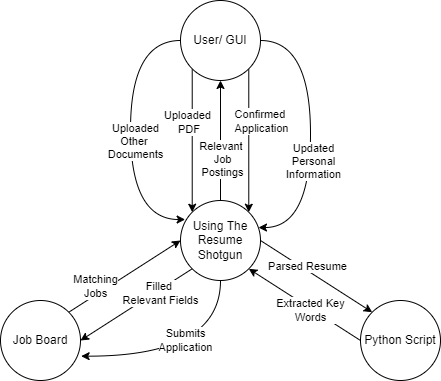
\includegraphics[width=125mm,scale=0.5]{SRS_Diagrams/SRS_Context_3.png}
    \caption{Work Context Diagram}
    \label{fig:context}
\end{figure}

\FloatBarrier

\begin{table}[ht]
\subsubsection{Work Partitioning}
\centering
    \begin{tabular}{|P{0.2in}|P{1.1in}|P{1.8in}|P{2.2in}|}
    \hline
    \textbf{\#} & \textbf{Event Name} & \textbf{Input/Output} & \textbf{Summary}\\ 
    
    \hline
    
    & & & \\
    
    1 
    & User uploads resume 
    & PDF Document (in) \hspace{2in} List of Keywords (out)
    % \begin{tabular}[l]{@{}l@{}} \\ PDF Document (in) \\ List of Keywords (out)\end{tabular}
    & The user uploads their Resume in the form of a PDF and the system uses this information to extract and construct a list of key words/phrases. \\
    
    & & & \\
    
    2 
    & User uploads auxiliary document 
    & PDF Document (in)
    & The user uploads their cover letter, transcript, or similar document to be stored. \\
    
    & & & \\
    
    3
    & User edits information
    & Information text (in) 
    & The user inputs information to fill or overwrite personal information used to complete applications. \\
    
    & & & \\
    
    4
    & User edits search terms
    & Information text (in)
    & The user inputs information to fill or overwrite criteria used to decide whether a job is relevant to consider for user applications, and what websites to look in. \\
    
    & & & \\
    
    5
    & User starts search for job links 
    & PDF Document (in) \hspace{2in} List of jobs' information (out)
    & The requested job board(s) are searched for postings with matching key words. A list is returned to the user containing the links and basic information about the job. \\
    
    & & & \\
    
    \hline
    \end{tabular}
    %\caption{Work Partitioning Business Events}
\end{table}

\begin{table}[ht]
\centering
    \begin{tabular}{|P{0.2in}|P{1.1in}|P{1.8in}|P{2.2in}|}
    \hline
    \textbf{\#} & \textbf{Event Name} & \textbf{Input/Output} & \textbf{Summary}\\ 
    
    \hline
    
    & & & \\
    
    6
    & User accepts recommended job posting 
    & Signal to apply on job board (out)
    & Job posting gets accepted by the user and the user information is automatically sent to the job board. \\
    
    & & & \\
    
    7
    & User rejects recommended job posting 
    &  Signal to disregard job posting (out)
    & Information gets removed from posting and the position is \textit{not} sent an application. \\
    
    & & & \\
    
    \hline
    \end{tabular}
    \caption{Work Partitioning Business Events}
\end{table}

\FloatBarrier

\subsubsection{Individual Product Use Cases}
%\textbf{Update if there is anything else to add} % this is a reminder to eventually remove this text
\begin{figure}[ht]
    \centering
    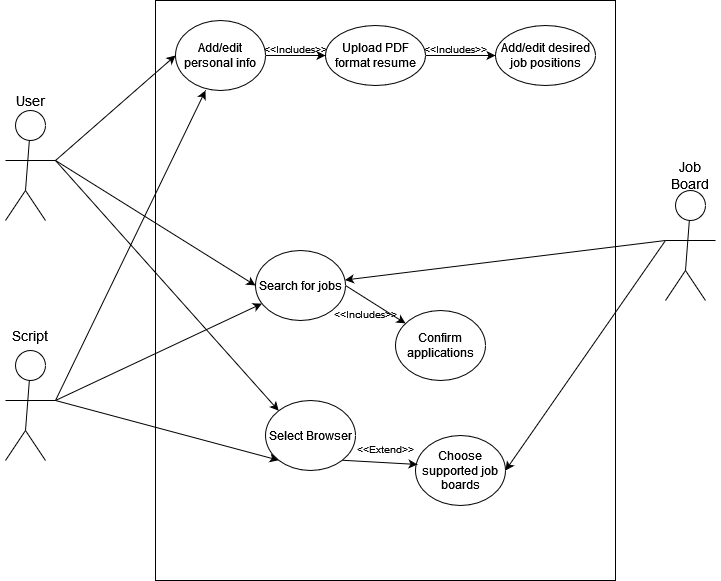
\includegraphics[width=125mm,scale=0.5]{SRS_Diagrams/3XA3useCase0.drawio.png}
    \caption{Use Case Diagram}
    \label{fig:usecase}
\end{figure}

\FloatBarrier

\subsection{Functional Requirements}

\begin{itemize}
    \item [FR1] The product shall allow the user to input information about themselves.
	{\newline \emph{Rationale}: Job applications require information about applicants.  
	\newline \textbf{Fit Criterion}: The product shall contain a list internally of every information field needed for the supported websites, and allow the user to fill in the blanks of the self-profile.}
	
    \item [FR2] The product shall be able to interact with PDF files designated by the user.
	{\newline \emph{Rationale}: The product needs to be able to extract keywords from the resume. Additionally, it needs to be able to upload PDF files to application websites, and PDF files are usually, if not always, accepted.    
	\newline \textbf{Fit Criterion}: When the user inputs their personal information in text form, the product shall also allow the user to also select any relevant files that may be needed for a job application. Additionally, it shall store this PDF file so it can be recalled later to be uploaded to websites.}
	
	\item [FR3] The product shall store user information, including after it has been stopped. 
	{\newline \emph{Rationale}: If the user is applying to multiple sites or across multiple days, inputting all the information each time is working against the goal of the product. 
	\newline \textbf{Fit Criterion}: The product shall store a profile on the user from the information they have inputted. It shall allow it to be both read and written to so the product can use it to fetch information for applying, and the user can update their profile.}
	
	\item [FR4] The product shall allow the user to select what websites to search for job openings on. 
	{\newline \emph{Rationale}: The user should be able to have control over their search; the user should be able to only search on websites they like.
	\newline \textbf{Fit Criterion}: When the user inputs their information, the product shall also allow the user to select as many websites from the list of supported websites as they like.}
	
	\item [FR5] The product shall allow the user to specify search terms for identifying jobs of interest. 
	{\newline \emph{Rationale}: In order for the provided information to be effective in landing the user a job, the jobs need to be related to the user.
	\newline \textbf{Fit Criterion}: When the user inputs their information, the product shall also allow the user to set up a "profile" for the job openings they are trying to find.}
	
	\item [FR6] The product shall allow the user to trigger a process that uses previously stored information to apply for jobs. 
	{\newline \emph{Rationale}: The purpose of the product; convenient and fast job applications.
	\newline \textbf{Fit Criterion}: After user information has been provided, have a trigger that starts the job scraping process.}
	
	\item [FR7] The product shall maintain a list of all jobs it has found, as well as applied to. 
	{\newline \emph{Rationale}: If the product is used across multiple sites or multiple times on the same site in the short term, it should try and prevent multiple applications to the same job.
	\newline \textbf{Fit Criterion}: The product shall maintain a list of jobs it has found and have them marked separately for if they were found but not used, or found and applied to. When doing subsequent job searches, the product shall reference this list to see if a job has previously been applied to. The product shall also raise warnings for the user to investigate if it finds jobs with similar descriptions and companies on different websites, as although the link would be different, the job might be the same.}
	
	\item [FR8] The product shall allow the user to preview job openings before automatically applying. 
	{\newline \emph{Rationale}: The user should have control over their search. The product could therefore also be used only to scrape for jobs as opposed to applying immediately. Additionally, the user should be able to avoid applying to jobs they do not like that they did not anticipate finding.
	\newline \textbf{Fit Criterion}: Between the points of scraping for job openings and submitting the applications, the product shall present the links and basic job information to the user so they can review what jobs they are going to apply for. They could then cancel automatic applications for jobs they may be interested in spending more time applying to, or want to avoid applications for altogether.}
\end{itemize}

\section{Non-functional Requirements}

\subsection{Look and Feel Requirements}
% should feel better than applying manually
\begin{itemize}
    \item [LF1] The system shall be easily readable with ASCII text through the command line that sufficiently displays all information.
    {\newline \emph{Rationale}: Accurate information is necessary for proper job applications, being able to read the output of the system is necessary for user success.
	\newline \textbf{Fit Criterion}: Variety of testers will be used to test out the visibility/ look of the final product and its interfacing.}
\end{itemize}

\subsection{Usability and Humanity Requirements}
\begin{itemize}
    \item [UH1] \itemlabel{item:UH1}{UH1} The product will only require identifying data and a resume to ensure a no discriminatory application process. The system will not inquire about sex, race, religion, age, and or genetic conditions.
    {\newline \emph{Rationale}: Sensitive user information as listed above is morally wrong and illegal to ask for in a job application.
	\newline \textbf{Fit Criterion}: No user input will be related to any potential discriminatory information.}
\end{itemize}

\subsection{Performance Requirements}
\begin{itemize}
    \item [PR1] The product shall be efficient in searching and matching up to 100 jobs in an acceptable amount of time of 5 minutes. 
    {\newline \emph{Rationale}: Having minimal response time for job applications is important since this product is specifically designed to be efficient and reduce the manual labour required for extended amounts of applications.
	\newline \textbf{Fit Criterion}: Measuring the time between the user's job search to match of a single job will be tested thoroughly and incremented to larger amount of jobs.}
	
\end{itemize}
\subsection{Operational and Environmental Requirements}
\begin{itemize}

    \item [OE1] \itemlabel{item:OE1}{OE1} The product should be executable on accessible modern operating systems such as Windows 10/11, MacOS and Linux.
    {\newline \emph{Rationale}: These are the most common operating systems currently being used on modern machines like laptops and desktops.
	\newline \textbf{Fit Criterion}: The product will be tested on all listed OS using personal and University provided resources.}
	
	\item [OE2] The product should be supported on the most accessible browsers; Chrome, Safari and Firefox.
	{\newline \emph{Rationale}:  These browsers are supported by one if not more OS as described in \ref{item:OE1} and used frequently.
	\newline \textbf{Fit Criterion}: The product will be tested on such browsers using personal and University provided resources.}
	
	\item [OE3] The product should be built and run with Python 3.
	{\newline \emph{Rationale}: Python 3 has great developer and user support as well as plenty of free libraries to use.
	\newline \textbf{Fit Criterion}: The team will follow a rigorous development cycle using Python 3.}
\end{itemize}	
	
\subsection{Maintainability and Support Requirements}
\begin{itemize}
    \item [MS1] All code will be publicly available and documented thoroughly.
	{\newline \emph{Rationale}: Thorough documentation allows developers to efficiently edit and maintain the well explained code.
	\newline \textbf{Fit Criterion}: All deadlines and revisions will be made public following the team's commitment to effective documentation.}
	
\end{itemize}


\subsection{Security Requirements}

\begin{itemize}
    \item [SR1] The product shall respect the user's privacy of personal information.
	{\newline \emph{Rationale}: The user should be aware of what is being done with their information; manual applications have this security feature so it should not be overlooked if automated.  
	\newline \textbf{Fit Criterion}: For every website being used, ask the user if they have read the privacy and release of information policies before releasing information to the job boards for applications. Provide links to said policies so they can be easily accessed if the user wants to read them.}
\end{itemize}

\subsection{Cultural Requirements}
\begin{itemize}
    \item [] See Usability and Humanity Requirement \ref{item:UH1}.
\end{itemize}

\subsection{Legal Requirements}

\begin{itemize}
    \item [LR1] Product will require thorough consent to necessary terms and conditions of applying on various job boards and personal information sharing.
	{\newline \emph{Rationale}: The user needs to be aware of job boards' intentions and their application process in using their website.
	\newline \textbf{Fit Criterion}: The team will thoroughly create accounts for the supported job boards and read all terms and conditions that will be necessary to share with the user.}
\end{itemize}
	
\subsection{Health and Safety Requirements}

N/A
% This section is not in the original Volere template, but health and safety are issues that should be considered for every engineering project.

\section{Project Issues}
% supersection

\subsection{Open Issues}

There are no known open issues.

\subsection{Off-the-Shelf Solutions}

This product is built off of an existing job application script (\href{https://github.com/harshibar/common-intern}{found here}), so there are similar, previously-existing products. However, the user has less control in the original product and it is not friendly for those unfamiliar working at lower than surface level with software.

There are also job application bots on the market (such as \href{https://www.websautomation.com/jobs-board-bot/}{these ones}), but these appear to be subscription based, sometimes costing upwards of \$100 per year - this is not ideal for our audience, who likely want to avoid spending money to land a job. % Probably important to include, I don;t know if it goes here

\subsection{New Problems}

In upgrading the original script, we now have the challenge of developing an intuitive way to interface with all of the configuration options. This also needs to be in a way that improves over the existing user interaction, as in it's original form it is not very accessible to those without some knowledge of code.

A very challenging part, obtaining all the information from a website to then use in a program, was done in the original script. However, this was done only for one site - other sites may still prove difficult despite having a working base to go off of. Furthermore, this does not account for differences between browsers.

\subsection{Tasks}

All tasks to complete for this project are outlined in the 
\href{https://gitlab.cas.mcmaster.ca/jamesong/application_3xa3_l01_grp05/-/tree/main/ProjectSchedule}{Gantt Chart} developed in the planning stage. 

\subsection{Migration to the New Product}

The original code is commented fairly well, but does not include proper test cases. For that reason, the original script will likely have parts rewritten for continuity or following conventions, but will largely stay and serve as the base for the new product. The original components will have tests created for them along with the new components being written.

\subsection{Risks}

The product adds no new risks otherwise specified within the terms and services of specific job board websites since it is a merely an automated tool for applying to positions more efficiently.

\subsection{Costs}

There are no costs associated with using/developing this product apart from computer and OS requirements. All software, libraries, job boards and browsers are free to use. However, some job boards allow for a premium subscriptions to be purchased. This product will not support any features from these paid subscriptions to ensure the costs are kept to a minimum and the product is available to as many users as possible. It is to note however that certain OS like Windows 10/11 and MacOS require a purchase of a specific device or the OS itself for use.

\subsection{User Documentation and Training}

The team will continuously use Doxygen to create well documented code that can be easily interpreted by those with a limited technical background. All revisions of the SRS will be made public. The product will include some direction to the user to guide them through use.

\subsection{Waiting Room}

N/A 

\subsection{Ideas for Solutions}

\begin{itemize}
    \item Similar to the original script, to avoid privacy concerns, the user will need to "prepare" the browser pages before activating the script. This means opening all of the job boards they want to search on, and logging in where applicable. This way, the product does not need to store login information.
    \item It is still unclear as to the most efficient way of dealing with PDF documents, but there have been a few options identified. Certain Python libraries allow files to be uploaded to a script (for example \href{https://pythonguides.com/upload-a-file-in-python-tkinter/}{Tkinter}), or the script could simply store the path to the PDF.
    \item For storing user information, making use of a YML file could be helpful, as it allows reading/writing both inside and outside the program. Using such a file may necessitate use of a library such as \href{https://pypi.org/project/PyYAML/}{PyYAML}.
    \item To take on the portability issues (including access to Python and OS), our Python project could be compiled into an EXE file (using resources listed \href{https://stackoverflow.com/questions/12059509/create-a-single-executable-from-a-python-project}{here}).
    \item Dealing with PDF files can be done with the \href{https://pypi.org/project/PyPDF2/}{PyPDF2} library, including which allows extracting document information and splitting documents by page.
    \item To make the product more intuitive to use, potentially expanding the user geographic, a GUI could be implemented (Tkinter, mentioned above, also works as a Python GUI). This would also allow easier viewing of all the information and files you have uploaded to be used.
\end{itemize}

\bibliographystyle{plainnat}

\bibliography{SRS}

\newpage

\section{Appendix}

% This section has been added to the Volere template.  This is where you can place additional information.

\subsection{Symbolic Parameters}

% The definition of the requirements will likely call for SYMBOLIC\_CONSTANTS. Their values are defined in this section for easy maintenance.

% None exist yet?

N/A

\newpage

\begin{table}[hp]
\caption{\bf Revision History}
\begin{tabularx}{\textwidth}{p{3cm}p{2cm}X}
\toprule {\bf Date} & {\bf Version} & {\bf Notes}\\
\midrule
Feb 8 & 0.1 & Sections and subsections 1, 2.2\\
Feb 10 & 0.2 & Fill of all remaining sections\\
\bottomrule
\end{tabularx}
\end{table}

\end{document}